%Copyright 2014 Jean-Philippe Eisenbarth
%This program is free software: you can 
%redistribute it and/or modify it under the terms of the GNU General Public 
%License as published by the Free Software Foundation, either version 3 of the 
%License, or (at your option) any later version.
%This program is distributed in the hope that it will be useful,but WITHOUT ANY 
%WARRANTY; without even the implied warranty of MERCHANTABILITY or FITNESS FOR A 
%PARTICULAR PURPOSE. See the GNU General Public License for more details.
%You should have received a copy of the GNU General Public License along with 
%this program.  If not, see <http://www.gnu.org/licenses/>.

%Based on the code of Yiannis Lazarides
%http://tex.stackexchange.com/questions/42602/software-requirements-specification-with-latex
%http://tex.stackexchange.com/users/963/yiannis-lazarides
%Also based on the template of Karl E. Wiegers
%http://www.se.rit.edu/~emad/teaching/slides/srs_template_sep14.pdf
%http://karlwiegers.com
\documentclass[12pt]{scrreprt}
%\documentclass{article}
\usepackage{listings}
\usepackage{booktabs}
\usepackage{underscore}
\usepackage{multirow}
\usepackage[bookmarks=true]{hyperref}
\usepackage[utf8]{inputenc}
\usepackage{graphicx}
\usepackage{diagbox}
\usepackage[english]{babel}
\usepackage{CJKutf8}
\usepackage{cite}
\usepackage{indentfirst} %首行縮排
\hypersetup{
    bookmarks=false,    % show bookmarks bar?
    pdftitle={Software Requirement Specification},    % title
    pdfauthor={Jean-Philippe Eisenbarth},                     % author
    pdfsubject={TeX and LaTeX},                        % subject of the document
    pdfkeywords={TeX, LaTeX, graphics, images}, % list of keywords
    colorlinks=true,       % false: boxed links; true: colored links
    linkcolor=blue,       % color of internal links
    citecolor=black,       % color of links to bibliography
    filecolor=black,        % color of file links
    urlcolor=purple,        % color of external links
    linktoc=page            % only page is linked
}%
\def\myversion{1.0 }
\date{}
%\title
\renewcommand{\tablename}{表} % 在文章中 table caption 會以「表 x」表示
\renewcommand{\figurename}{圖} % 在文章中 figure caption 
\renewcommand{\baselinestretch}{1.5} 

% 全部行距皆為 20 points
\CJKencfamily{UTF8}{bkai} % 使用標楷體
\AtBeginDocument{%
    \begin{CJK}{UTF8}{bkai}} % 使用標楷體
    \AtEndDocument{%
    \clearpage\end{CJK}}
\makeatother

\usepackage{hyperref}
\begin{document}

\CJKindent
\begin{center}
 %   \rule{16cm}{5pt}\vskip1cm
    \begin{bfseries}
        \Huge{基於即時情緒分析之心靈陪伴系統}\\
         \vspace{2cm}
		開放平台期末專題\\
	 \vspace{2cm}
         {\huge組長\\}
		{\huge1043335 賴詩雨\\}
	\vspace{1cm}
         {\huge組員\\}
		{\huge1041419 蔡怡君\\
		1041529 龐渝庭\\
		1043338 蔡昕芸\\
		1043341 吳悅琳\\}
	\vspace{2cm}
		{\huge\today\\}
%        for\\
%        \vspace{1.9cm}
%        $<$Project$>$\\
%        \vspace{1.9cm}
%        \LARGE{Version \myversion approved}\\
%        \vspace{1.9cm}
%        Prepared by $<$author$>$\\
%        \vspace{1.9cm}
%        $<$Organization$>$\\
%        \vspace{1.9cm}
%        \today\\
    \end{bfseries}
\end{center}

\tableofcontents


\chapter*{Revision History}

\begin{center}
    \begin{tabular}{|c|c|c|c|}
        \hline
	    Name & Date & Reason For Changes & Version\\
        \hline
	    蔡昕芸、蔡怡君 & 6/15 & 新增各項內容大綱 & 1\\
        \hline
	    蔡怡君 & 6/21 & 內容修改 & 2.1\\
        \hline
	    蔡昕芸、吳悅琳 & 6/21 & 內容修改 & 2.2\\
        \hline
	    31 & 6/22 & 內容修改 & 3\\
        \hline
    \end{tabular}
\end{center}
\chapter{產品介紹}

\section{目的}

現代人工作忙碌、生活步調快,容易產生緊張、焦慮等非正向情緒。研究顯示長久處於非正向情緒,可能造成身體器官的損壞,而罹患某些疾病,例如:癌症、憂鬱症和躁鬱症等。為了解決此問題,本團隊提出一基於即時情緒分析之心靈陪伴系統,透過攝影機,拍攝病人臉部影像,並快速辨識使用者是否處於非正向的情緒。同時,即時線上搜尋改善病人當下情緒的音樂播放,並且以語音方式播放可以緩和情緒的心靈小語,藉此使病人心靈得到安慰。除此之外,本產品也提供心靈陪伴分析平台,讓使用者可以查看過去所有非正向情緒的累積統計圖,以及非正向情緒可能導致的相關疾病,去做提醒跟建議。

另外,在心靈陪伴分析平台中,也提供使用者留言板,我們會根據病人的留言內容,去做客製化的分析,針對病人的問題去修改回應內容,使回應能更符合病人的需要。況且,這些內容是不會對外公開的,病人不須擔心隱私被洩露。

%\section{文件公約} %應該不用寫
%$<$Describe any standards or typographical conventions that were followed when 
%writing this SRS, such as fonts or highlighting that have special significance.  
%For example, state whether priorities  for higher-level requirements are assumed 
%to be inherited by detailed requirements, or whether every requirement statement 
%is to have its own priority.$>$

\section{預期讀者和閱讀建議}
%$<$ Describe the different types of reader that the document is intended for, 
%such as developers, project managers, marketing staff, users, testers, and 
%documentation writers. Describe what the rest of this SRS contains and how it is 
%organized. Suggest a sequence for reading the document, beginning with the 
%overview sections and proceeding through the sections that are most pertinent to 
%each reader type.$>$

本SRS文件提供給使用者、開發團隊與維護人員閱讀,使用者透過閱讀本文件,了解產品以及操作說明,開發團隊進行系統開發時的依據,與維護人員日後維護系統時的參考文件。

\section{計畫範圍}
與其他章節有所重複,請參考文件1.1。
%$<$Provide a short description of the software being specified and its purpose, 
%including relevant benefits, objectives, and goals. Relate the software to 
%corporate goals or business strategies. If a separate vision and scope document 
%is available, refer to it rather than duplicating its contents here.$>$

%此文件的範圍是針對「心靈陪伴分析」之軟體需求規格,包括系統前端(Client端)及系統後端(Server端)的相關架構與功能。

\section{參考資料}
\begin{itemize}
\item{http://big5.gov.cn/gate/big5/www.gov.cn/fwxx/kp/2008-01/17/content_861306.htm}

\item{https://www.cw.com.tw/article/article.action?id=5081933}

\item{http://www.alternative-cancer-care.com/cancer-anger-link.html}

\item{https://www.cancer.gov/about-cancer/coping/feelings/stress-fact-sheet}

\item{https://newsinhealth.nih.gov/2015/08/positive-emotions-your-health}
\end{itemize}
%$<$List any other documents or Web addresses to which this SRS refers. These may include user interface style guides, contracts, standards, system requirements specifications, use case documents, or a vision and scope document. Provide enough information so that the reader could access a copy of each reference, including title, author, version number, date, and source or location.$>$


\chapter{總體描述}

\section{產品透視} %components diagram
$<$Describe the context and origin of the product being specified in this SRS.  
For example, state whether this product is a follow-on member of a product 
family, a replacement for certain existing systems, or a new, self-contained 
product. If the SRS defines a component of a larger system, relate the 
requirements of the larger system to the functionality of this software and 
identify interfaces between the two. A simple diagram that shows the major 
components of the overall system, subsystem interconnections, and external 
interfaces can be helpful.$>$

\section{產品功能} %class diagram
%$<$Summarize the major functions the product must perform or must let the user 
%perform. Details will be provided in Section 3, so only a high level summary 
%(such as a bullet list) is needed here. Organize the functions to make them 
%understandable to any reader of the SRS. A picture of the major groups of 
%related requirements and how they relate, such as a top level data flow diagram 
%or object class diagram, is often effective.$>$
本系統主要是針對病人去做情緒偵測,並且當下立即利用播放音樂、回應話去舒緩病人的非正向情緒,每一次的情緒都會儲存在後端的database裡面,病人可以透過我們心靈陪伴分析平台網頁,去了解自己每天的情緒和全部的情緒統計,搭配貼心小建議可以更清楚需要注意的身體狀況。另外,我們還設置留言板供用戶可以抒發或者分享自己的心情,所有內容一律保密,不會外流,請用戶放心。

\section{用戶類別和特質}
我們的系統用戶,針對正在接受治療的病人,如︰憂鬱症、癌症等,利用攝影機拍攝病人的臉部影像,辨識是否處於非正向情緒,如︰焦慮、憤怒等,播放語音回應及線上音樂,緩和病人情緒,並且可利用心靈陪伴分析平台網頁,網頁中提供病人的情緒數據、建議事項及心情留言板,藉此了解、調適個人心理狀態,輔助病人情緒達到穩定,使病情能更快速康復。
%$<$Identify the various user classes that you anticipate will use this product. User classes may be differentiated based on frequency of use, subset of product functions used, technical expertise, security or privilege levels, educational level, or experience. Describe the pertinent characteristics of each user class.  Certain requirements may pertain only to certain user classes. Distinguish the most important user classes for this product from those who are less important to satisfy.$>$

\section{操作環境}
%$<$Describe the environment in which the software will operate, including the 
%hardware platform, operating system and versions, and any other software 
%components or applications with which it must peacefully coexist.$>$

\subsection{軟體需求}
\begin{itemize}
\item[(1)]{\begin{bfseries}{操作系統:}Windows 10\end{bfseries}}
\item[(2)]{\begin{bfseries}{程式撰寫平台:}Pycharm 2016.3.2\end{bfseries}}
\item[(3)]{\begin{bfseries}{操作環境:}Python3.5.0 以上\end{bfseries}}
%%網頁端要加
\end{itemize}

\subsection{硬體需求}
\begin{itemize}
\item[(1)]{\begin{bfseries}{音響:}外接藍芽喇叭或電腦內建喇叭\end{bfseries}}
\item[(2)]{\begin{bfseries}{攝影鏡頭:}USB2.0外接攝影鏡頭或電腦內建鏡頭\end{bfseries}}
\item[(3)]{\begin{bfseries}{網路:}無線網路卡或手機 wifi\end{bfseries}}

\end{itemize}

\section{設計和實作上的限制}
卷積神經網路的訓練集來源,因採用國外公開的臉孔資料庫,因此缺乏東方臉孔的數據。
%$<$Describe any items or issues that will limit the options available to the developers. These might include: corporate or regulatory policies; hardware limitations (timing requirements, memory requirements); interfaces to other applications; specific technologies, tools, and databases to be used; parallel operations; language requirements; communications protocols; security considerations; design conventions or programming standards (for example, if the customer’s organization will be responsible for maintaining the delivered software).$>$

\section{用戶文件}
$<$List the user documentation components (such as user manuals, on-line help, 
and tutorials) that will be delivered along with the software. Identify any 
known user documentation delivery formats or standards.$>$
\section{系統假設和依賴}

本產品使用的套件包含:NumPy、OpenCV、Tensorflow、Keras、BeautifulSoup、
youtube_dl、lxml、ffmpeg、pymongo、urllib、json、django,因此,當第三方套件停止服務時,我們的程式將無法運行。

%$<$List any assumed factors (as opposed to known facts) that could affect the 
%requirements stated in the SRS. These could include third-party or commercial 
%components that you plan to use, issues around the development or operating 
%environment, or constraints. The project could be affected if these assumptions 
%are incorrect, are not shared, or change. Also identify any dependencies the 
%project has on external factors, such as software components that you intend to 
%reuse from another project, unless they are already documented elsewhere (for 
%example, in the vision and scope document or the project plan).$>$


\chapter{界面規格設計}

\section{使用者介面}
%$<$Describe the logical characteristics of each interface between the software 
%product and the users. This may include sample screen images, any GUI standards 
%or product family style guides that are to be followed, screen layout 
%constraints, standard buttons and functions (e.g., help) that will appear on 
%every screen, keyboard shortcuts, error message display standards, and so on.  
%Define the software components for which a user interface is needed. Details of 
%the user interface design should be documented in a separate user interface 
%specification.$>$

我們將使用者介面分為兩個部份,包含︰情緒偵測介面及心靈分析平台介面,概述如下︰

在偵測使用者情緒時,我們利用電腦視窗的形式,顯示使用者臉部影像,呈現臉部偵測、偵測結果及臉部辨識後的情緒分析數據,如圖\ref{fig:UserInterface-1}所示。
\begin{figure}[!h]
\begin{center}
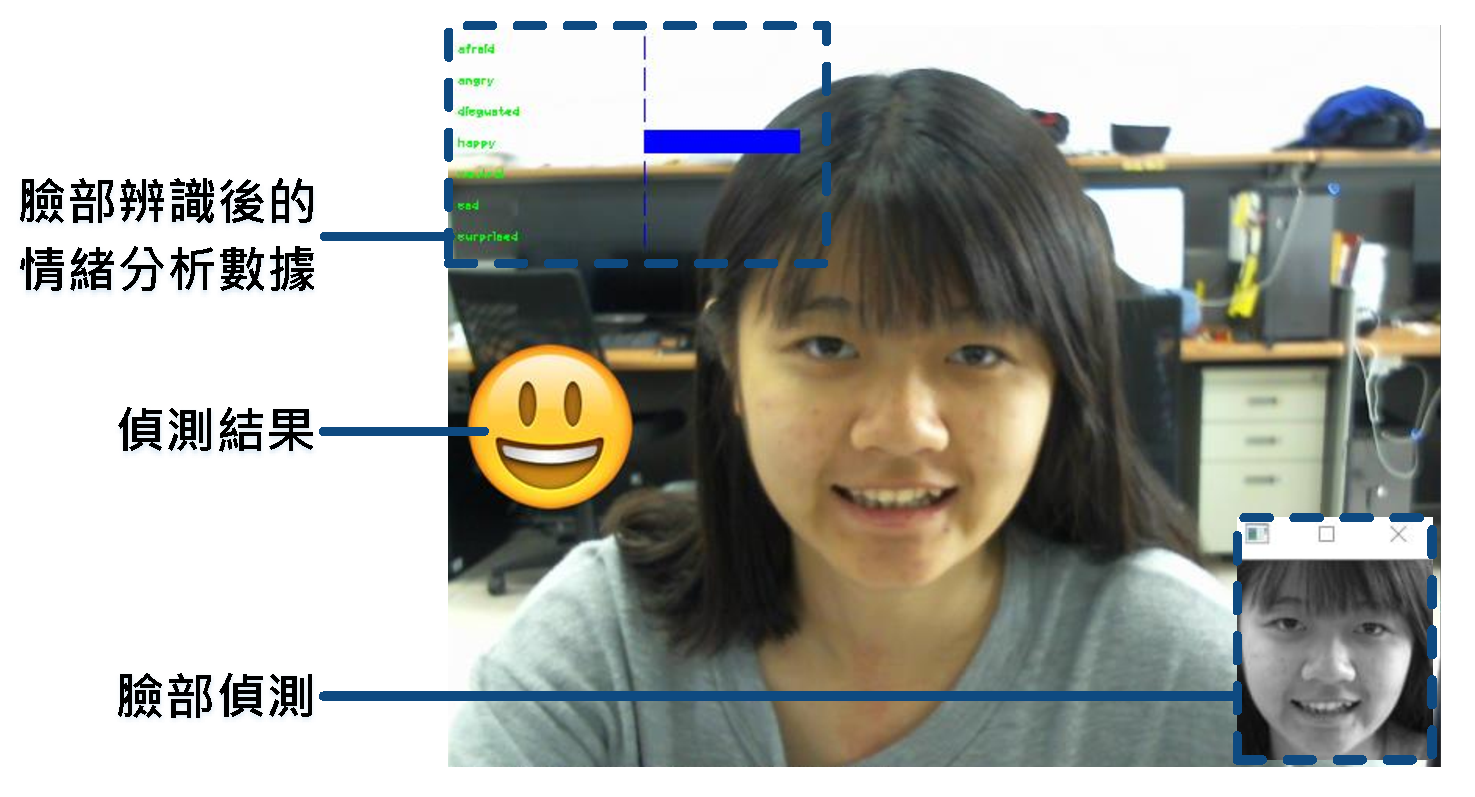
\includegraphics[width=0.7\textwidth]{./figs/DetectResult-2.pdf}
\end{center}
\caption{情緒偵測介面說明圖。}
\label{fig:UserInterface-1}
\end{figure}

在偵測完使用者的情緒後,我們透過網頁的形式,呈現情緒數據的直方圖,提供給病人查看,另外,網頁下方也提供貼心小建議與留言板,提醒病人注意心理狀態,以及讓病人留言抒發情緒,如圖\ref{fig:UserInterface-2}所示。

\begin{figure}[!h]
\begin{center}
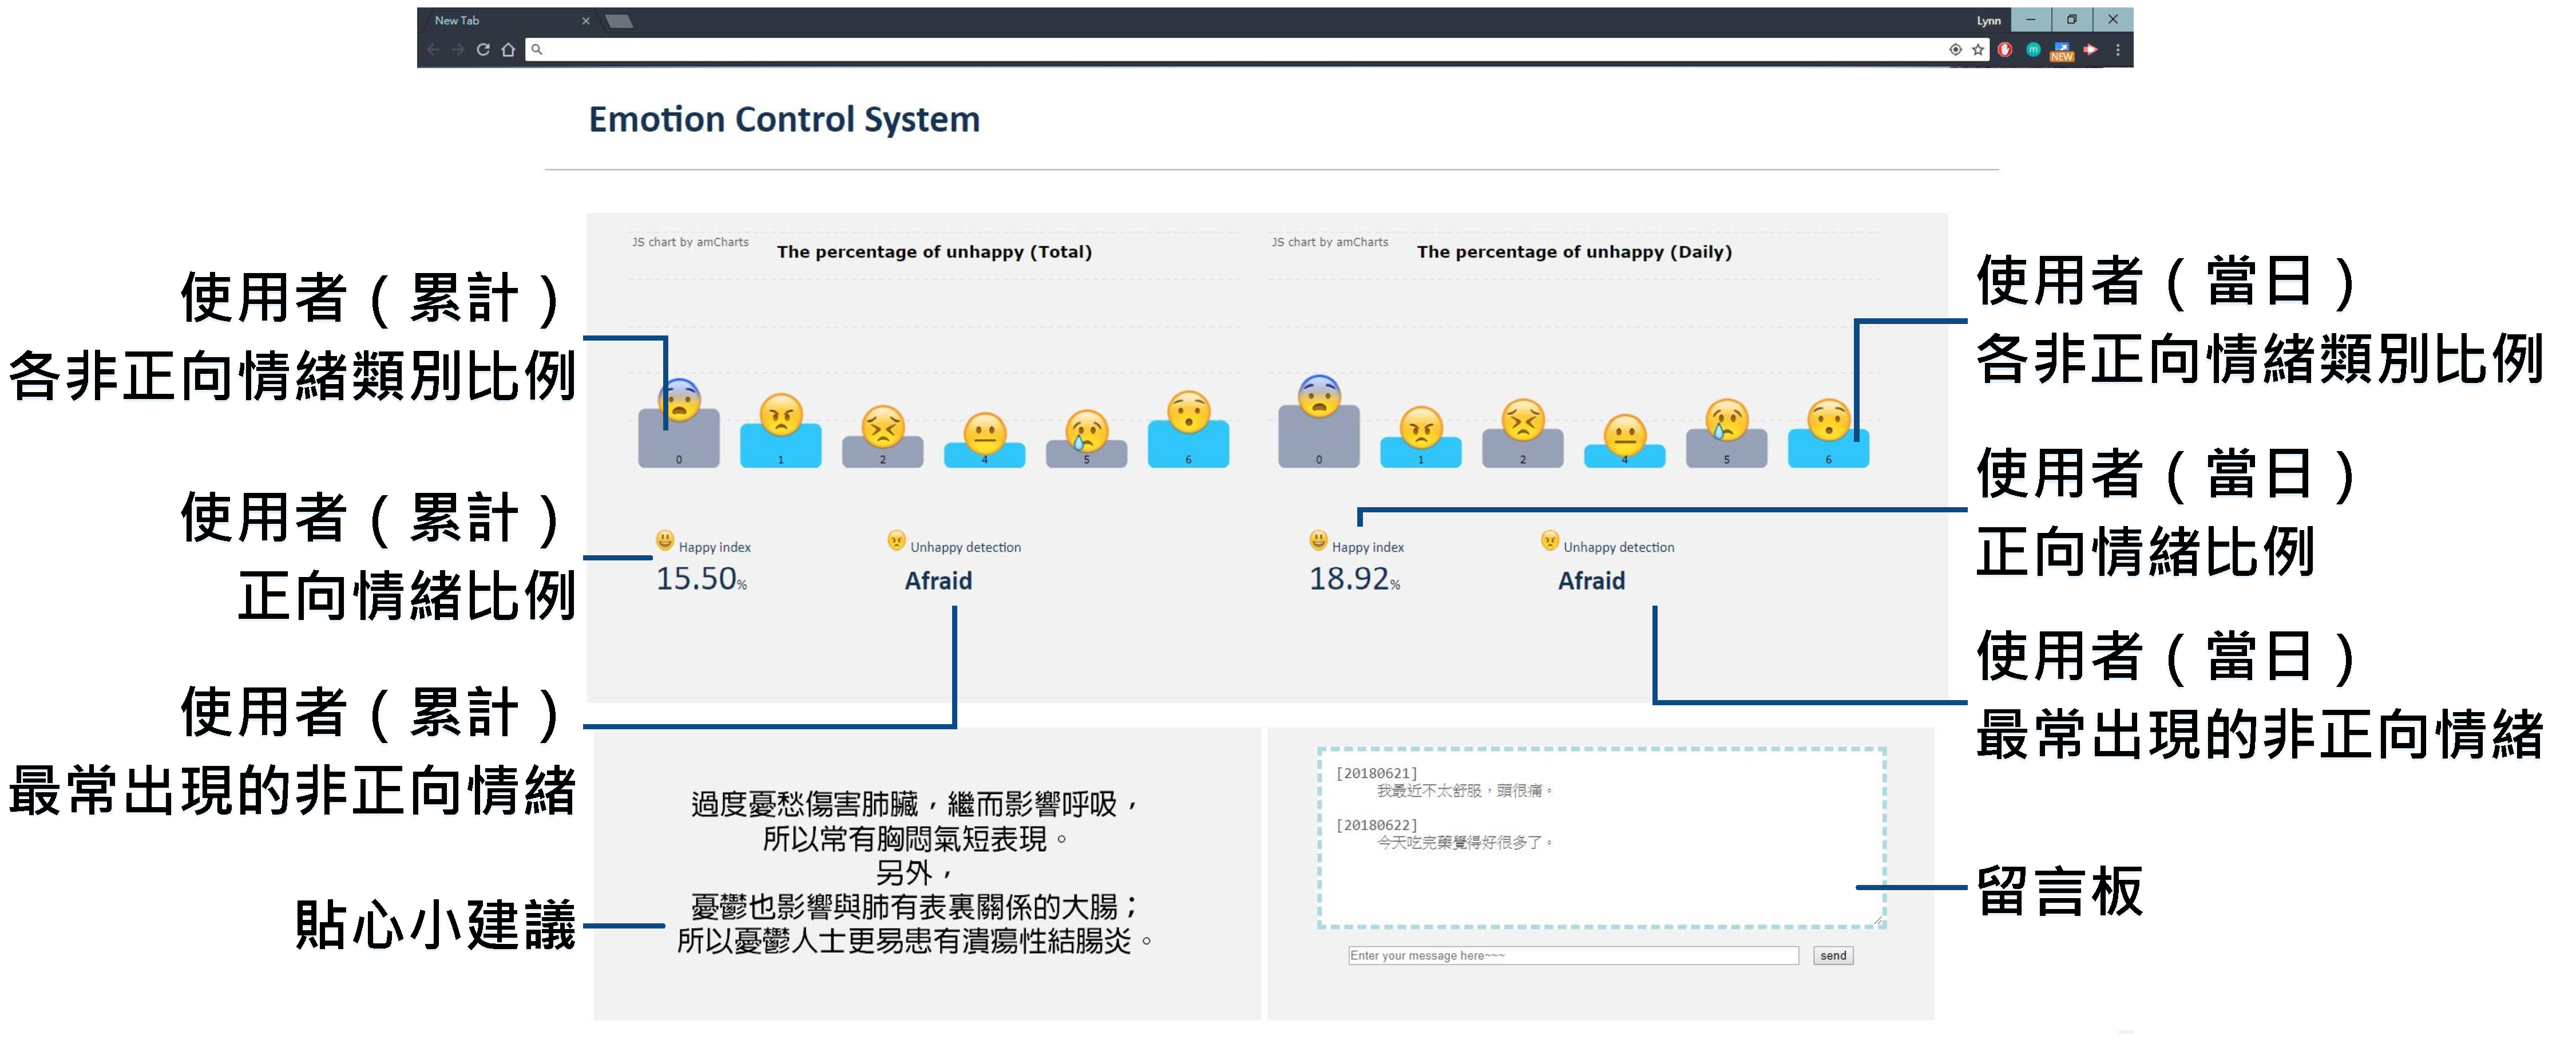
\includegraphics[width=1\textwidth]{./figs/Web.pdf}
\end{center}
\caption{心靈分析平台介面說明圖。}
\label{fig:UserInterface-2}
\end{figure}



\section{硬體界面}
本產品包含USB2.0外接攝影鏡頭、藍芽喇叭及音源線,將攝影鏡頭及藍芽喇叭分別插入電腦USB孔及音源孔,即可使用。另外,筆電本身含有攝影鏡頭的,則可不必在外接攝影鏡頭,如圖\ref{fig:hardInterface}。
\begin{figure}[!h]
\begin{center}
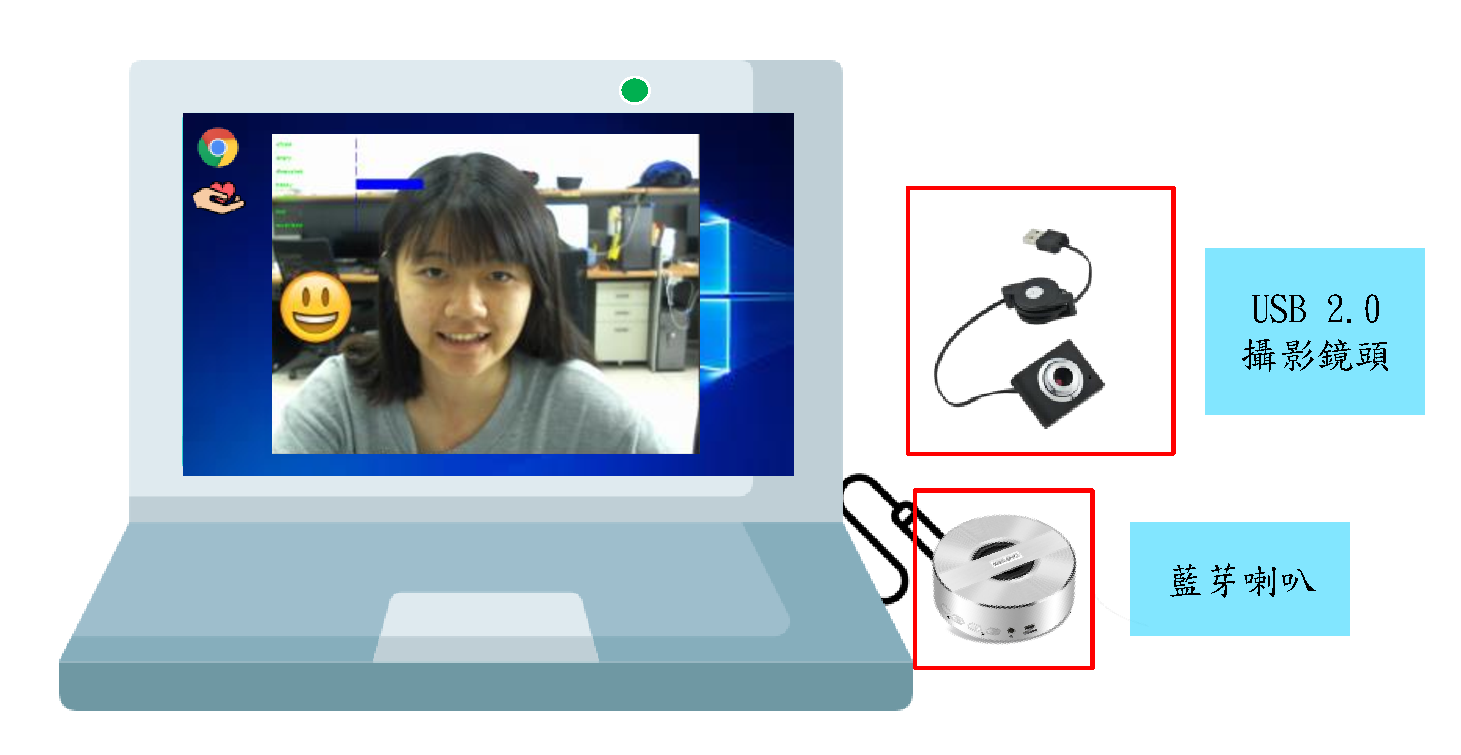
\includegraphics[width=0.8\textwidth]{./figs/hardware.pdf}
\end{center}
\caption{硬體界面說明圖。}
\label{fig:hardInterface}
\end{figure}
%$<$Describe the logical and physical characteristics of each interface between the software product and the hardware components of the system. This may include the supported device types, the nature of the data and control interactions between the software and the hardware, and communication protocols to be used.$>$硬體線路圖, 腳位, 訊號等資訊. 最好用Bloack diagram 的方式描述另外如能加上耗電量, 效能等資訊更好.

\section{軟體界面}
%$<$Describe the connections between this product and other specific software 
%components (name and version), including databases, operating systems, tools, 
%libraries, and integrated commercial components. Identify the data items or 
%messages coming into the system and going out and describe the purpose of each.  
%Describe the services needed and the nature of communications. Refer to 
%documents that describe detailed application programming interface protocols.  
%Identify data that will be shared across software components. If the data 
%sharing mechanism must be implemented in a specific way (for example, use of a 
%global data area in a multitasking operating system), specify this as an 
%implementation constraint.$>$
軟體的架構, 功能列表, 變數與函數的列表說明.

\section{通信界面}
$<$Describe the requirements associated with any communications functions 
required by this product, including e-mail, web browser, network server 
communications protocols, electronic forms, and so on. Define any pertinent 
message formatting. Identify any communication standards that will be used, such 
as FTP or HTTP. Specify any communication security or encryption issues, data 
transfer rates, and synchronization mechanisms.$>$


\chapter{系統功能}

根據國內〈科學發展〉期刊的相關研究發現,音樂可以產生催產素,以減低焦慮與恐懼,有效改善情緒,因此,本系統:基於即時情緒分析之心靈陪伴系統,應用於醫療系統的照護病患機制,本專案系統主要分為兩部份,分別為使用者端和伺服器端,使用者端為即時分析情緒及情緒緩和,包含情緒偵測演算法及情緒緩和機制,伺服器端則為後端平台做分析追蹤,包含雲端心靈陪伴分析整合平台,如圖\ref{fig:framework},概略說明如下:

%%%%圖要改
\begin{figure}[!h]
\begin{center}
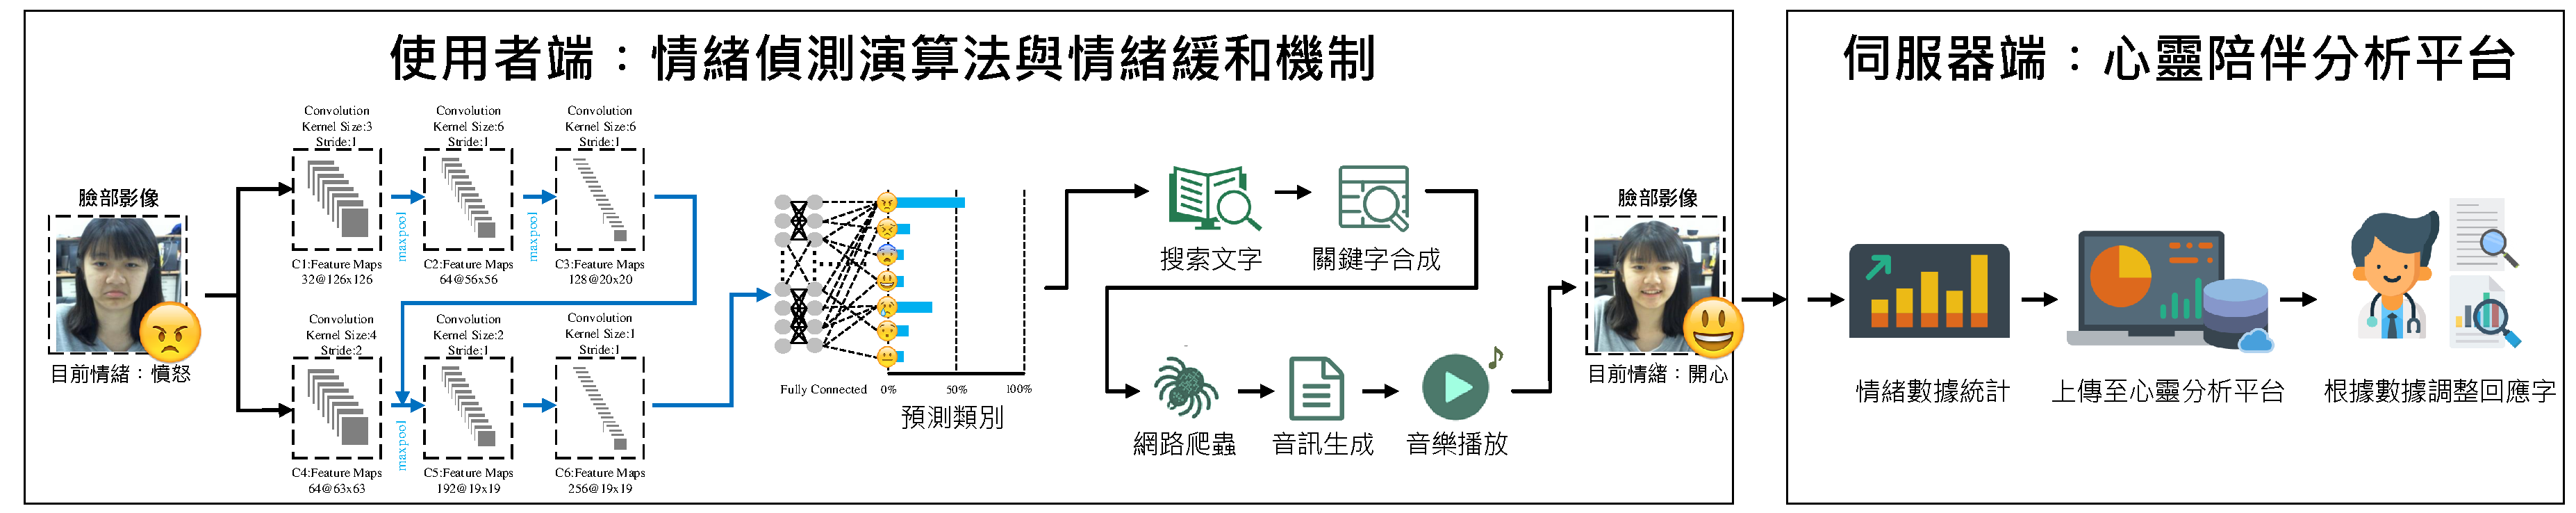
\includegraphics[width=1\textwidth]{./figs/framework-version2.pdf}
\end{center}
\caption{非接觸式準確且即時駕駛情緒偵測演算法架構圖。}
\label{fig:framework}
\end{figure}

\section{使用者端}

\subsection{即時分析情緒及情緒緩和}


\begin{itemize}
\item{\begin{bfseries}{情緒偵測演算法:}\end{bfseries}}

我們為避免病人因非正向情緒,持續影響心理、生理,進而導致不可預期的危害,我們利用深度學習的卷積神經網路CNN,由1個輸入層、6個卷積層(Convolution layer)、3個池化層(Pooling layer)、1個全連接層(Fully Connected)和1個輸出層所構成,來訓練情緒辨識模型,偵測病人情緒。由於情緒的時間性變化,我們亦進行兩階段的Voting機制,第一階段為篩選出病人可能的情緒,第二階段為避免病人因為短時間臉部抽動(如:打哈欠),導致誤判情緒,透過上述兩階段的Voting後,得出最準確的病人情緒判斷。\\

\item{\begin{bfseries}{情緒緩和機制:}\end{bfseries}}

透過情緒偵測演算法,得出的病人情緒後,即時抓取能有效改善病人當下情緒的音樂並播放,使病人情緒緩和,避免病人因非正向情緒,導致影響心理,使病情不易痊癒、影響治療過程。因此,我們分為五個步驟達成,包括:搜索文字、關鍵字合成、網路爬蟲、音訊生成、以及音樂播放等五個步驟。
\begin{itemize}
\item[(a)]{\begin{bfseries}{搜索文字:}\end{bfseries}}

如圖\ref{fig:FrameworkFirstAndSecond}右半部(a),當抓取到病人情緒後,我們隨機搜索一組預先設定的回應文字,如表\ref{lab:searchtext}所示,利用語音播放,回應正向語句,鼓勵病人。\\

\renewcommand{\arraystretch}{1.0} 
\renewcommand{\multirowsetup}{\centering}

\begin{table}[h]
\caption{搜索文字表}
    \centering
\begin{tabular}{|*{4}{r|}}
\hline
\multicolumn{1}{|c|}{情緒}
& \multicolumn{3}{c|}{回應字} \\\hline
\multicolumn{1}{|c}{憤怒}&\multicolumn{1}{|c}{奧特曼,你別氣了,…}&\multicolumn{1}{|c}{……}&\multicolumn{1}{|c|}{沒有什麼事情是十全…} \\\hline
\multicolumn{1}{|c}{悲傷}&\multicolumn{1}{|c}{讓我陪你一起面對,…}&\multicolumn{1}{|c}{……}&\multicolumn{1}{|c|}{我知道現在的你情緒…} \\\hline
\multicolumn{1}{|c}{驚嚇}&\multicolumn{1}{|c}{偉大的哈利來幫你了…}&\multicolumn{1}{|c}{……}&\multicolumn{1}{|c|}{你心裡一定很不好受…}\\\hline
\multicolumn{1}{|c}{憂慮}&\multicolumn{1}{|c}{如果你願意說,我隨…}&\multicolumn{1}{|c}{……}&\multicolumn{1}{|c|}{遇到什麼是很心煩嗎…}\\\hline
\multicolumn{1}{|c}{厭惡}&\multicolumn{1}{|c}{燒毀,燒毀,斷開魂…}   &\multicolumn{1}{|c}{……}   &\multicolumn{1}{|c|}{偶爾深呼吸,心情更… }\\\hline
\multicolumn{1}{|c}{無表情}&\multicolumn{1}{|c}{有一個爸爸帶四歲的…}   &\multicolumn{1}{|c}{……}   &\multicolumn{1}{|c|}{我來講個笑話給你聽…}\\\hline
\multicolumn{1}{|c}{開心}&\multicolumn{1}{|c}{你開心ya,我開心ya…}   &\multicolumn{1}{|c}{……}   &\multicolumn{1}{|c|}{今天心情不錯!繼續保…}\\\hline
\end{tabular}
\label{lab:searchtext}
\end{table}

\item[(b)]{\begin{bfseries}{關鍵字合成:}\end{bfseries}}

我們根據設定的查找表(Lookup Table)來合成網路爬蟲關鍵字,如表\ref{lab:2}所示(放關鍵字合成的表)。其中,如果是偵測到病人的情緒為「憤怒」,會查找到可能的關鍵字有「古典樂放鬆」、「古典樂輕快」、「流行歌輕快」等,以找尋放鬆、輕快的音訊資料,如圖\ref{fig:FrameworkFirstAndSecond}右半部(b)所示。\\

\renewcommand{\arraystretch}{1.0} 
\renewcommand{\multirowsetup}{\centering}
\begin{table}[h]
\caption{關鍵字合成表}
    \centering
\begin{tabular}{|*{4}{r|}}
\hline
\multicolumn{1}{|c|}{情緒}
& \multicolumn{3}{c|}{關鍵字} \\\hline
\multicolumn{1}{|c}{憤怒}&\multicolumn{1}{|c}{古典樂放鬆}&\multicolumn{1}{|c}{古典樂輕快}&\multicolumn{1}{|c|}{流行歌輕快} \\\hline
\multicolumn{1}{|c}{悲傷}&\multicolumn{1}{|c}{療癒音樂}&\multicolumn{1}{|c}{交響樂輕快}&\multicolumn{1}{|c|}{交響曲振奮} \\\hline
\multicolumn{1}{|c}{驚嚇}&\multicolumn{1}{|c}{鋼琴輕音樂}&\multicolumn{1}{|c}{背景音樂輕鬆}&\multicolumn{1}{|c|}{背景音樂抒情}\\\hline
\multicolumn{1}{|c}{厭惡}&\multicolumn{1}{|c}{純音樂提神}&\multicolumn{1}{|c}{交響樂震撼}&\multicolumn{1}{|c|}{背景音樂震撼}\\\hline
\multicolumn{1}{|c}{焦慮}&\multicolumn{1}{|c}{古典樂振奮}   &\multicolumn{1}{|c}{舒緩音樂}   &\multicolumn{1}{|c|}{振奮人心音樂}\\\hline
\multicolumn{1}{|c}{無表情}&\multicolumn{1}{|c}{背景音樂輕鬆}   &\multicolumn{1}{|c}{背景音樂抒情}   &\multicolumn{1}{|c|}{流行歌輕快}\\\hline
\multicolumn{1}{|c}{開心}&\multicolumn{1}{|c}{清音樂自然}   &\multicolumn{1}{|c}{鋼琴輕音樂}   &\multicolumn{1}{|c|}{背景音樂自然}\\\hline
\end{tabular}
\label{lab:2}
\end{table}

\item[(c)]{\begin{bfseries}{網路爬蟲:}\end{bfseries}}

利用關鍵字合成,使用網路爬蟲,抓取有效改善病人當下情緒的音樂,我們採用HTTP Request技術,以及requests、urllib2、 BeautifulSoup 、lxml、 youtube-dl等軟體開發套件,根據上述的關鍵字檢索結果,從網絡上抓取最新最即時的音訊資料,如圖\ref{fig:FrameworkFirstAndSecond}右半部(c)所示。\\

\item[(d)]{\begin{bfseries}{音訊生成:}\end{bfseries}}

當我們抓取到音訊資料後,通過Python的Requests及 BeautifulSoup技術,來下載檔案,使音訊生成,如圖\ref{fig:FrameworkFirstAndSecond}右半部(d)所示。\\

\item[(e)]{\begin{bfseries}{音樂播放:}\end{bfseries}}

當我們生成音訊資料後,使用omxplayer套件,將音訊播放給病人收聽,改善病人當下的情緒,如圖\ref{fig:FrameworkFirstAndSecond}右半部(e)所示。\\

根據以上五個步驟,即可完成情緒緩和機制,藉此避免病人因非正向情緒,導致影響病情,賦予病人積極、正面的動力。\\

\end{itemize}
\end{itemize}

\begin{figure}[!h]
\begin{center}
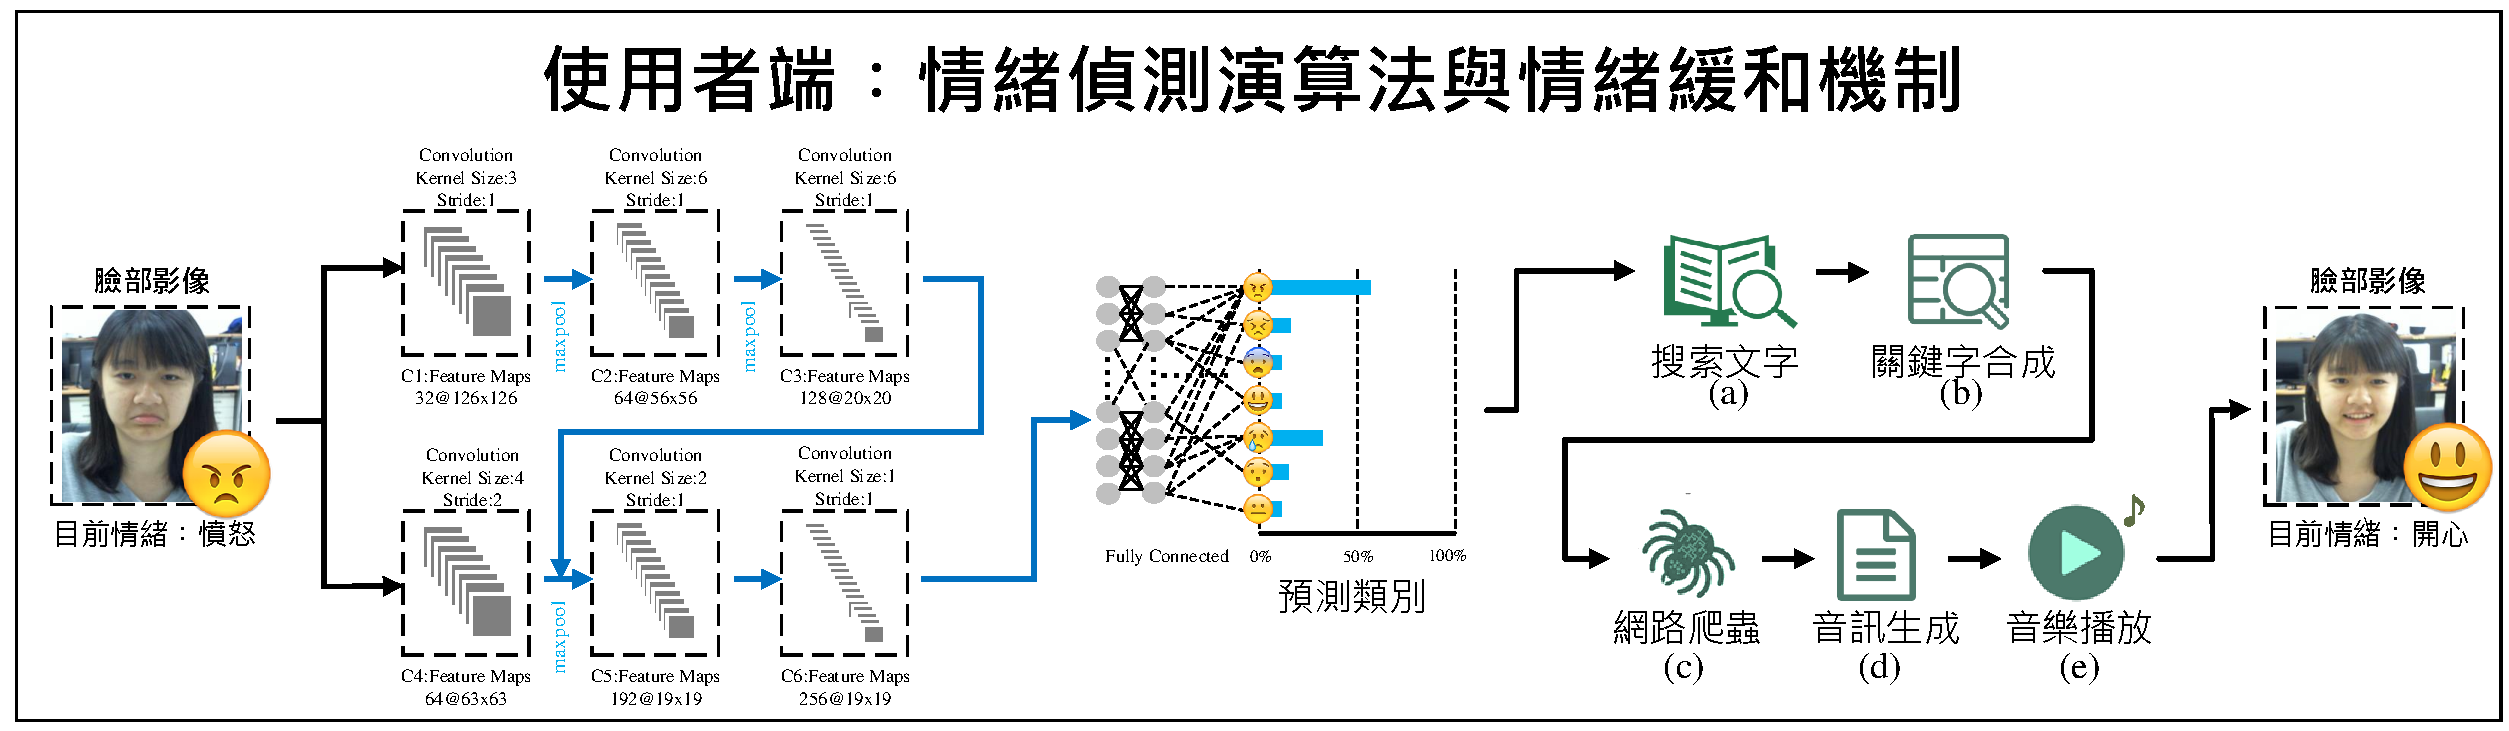
\includegraphics[width=1\textwidth]{./figs/FrameworkFirstAndSecond.pdf}
\end{center}
\caption{使用者端︰情緒偵測演算法與情緒緩和機制架構圖。}
\label{fig:FrameworkFirstAndSecond}
\end{figure}

\subsection{UML使用案例圖表}
$<$List the sequences of user actions and system responses that stimulate the 
behavior defined for this feature. These will correspond to the dialog elements 
associated with use cases.$>$

\subsection{功能性需求}

\begin{center}  
\begin{tabular}{|l| p{10cm}|}  
\hline  
功能性需求 & 功能性需求描述   \\ \hline  
情緒辨識 &以本系統介面偵測病人臉部表情,偵測7種表情,包含6種非正向情緒,如︰憂鬱、悲傷、憤怒、面無表情、厭惡、驚嚇等,及1種正向情緒,如︰開心。    \\ \hline  
搜索文字& 好的\\\hline
關鍵字合成 & 抓取到病人情緒後,根據設定的查閱表資料表,合成網路爬蟲關鍵字。例如:偵測到病人的情緒為憤怒,會查找到可的關鍵字有..「古典樂放鬆」、「古典樂輕快」、「流行歌輕快」等,以找尋放鬆、輕快的音訊資料    \\ \hline  
網路爬蟲 & 利用情緒關鍵字,抓取有效改善病人當下情緒的音樂 \\ \hline
音訊生成 & 抓取音訊資料後下載檔案,使音訊生成 \\ \hline
音樂播放 & 生成音訊後,將音訊播放給病人收聽,改善病人當下的情緒 \\ \hline

\end{tabular}  
\end{center}  


\section{伺服器端}

\subsection{後端平台做分析追蹤}
\begin{itemize}
\item{\begin{bfseries}{雲端心靈陪伴分析整合平台:}\end{bfseries}}
透過即時分析情緒及情緒緩和過後,我們導入分析後的非正向情緒類別,設計一雲端心靈陪伴分析整合平台,如圖\ref{fig:webframework}所示,以提供視覺化情緒統計的服務。如此一來,病人能透過網頁,查詢自己的歷史狀況,以及分析統計結果;查詢自己常處於哪類的非正向情緒...........。
\begin{figure}[!h]
\begin{center}
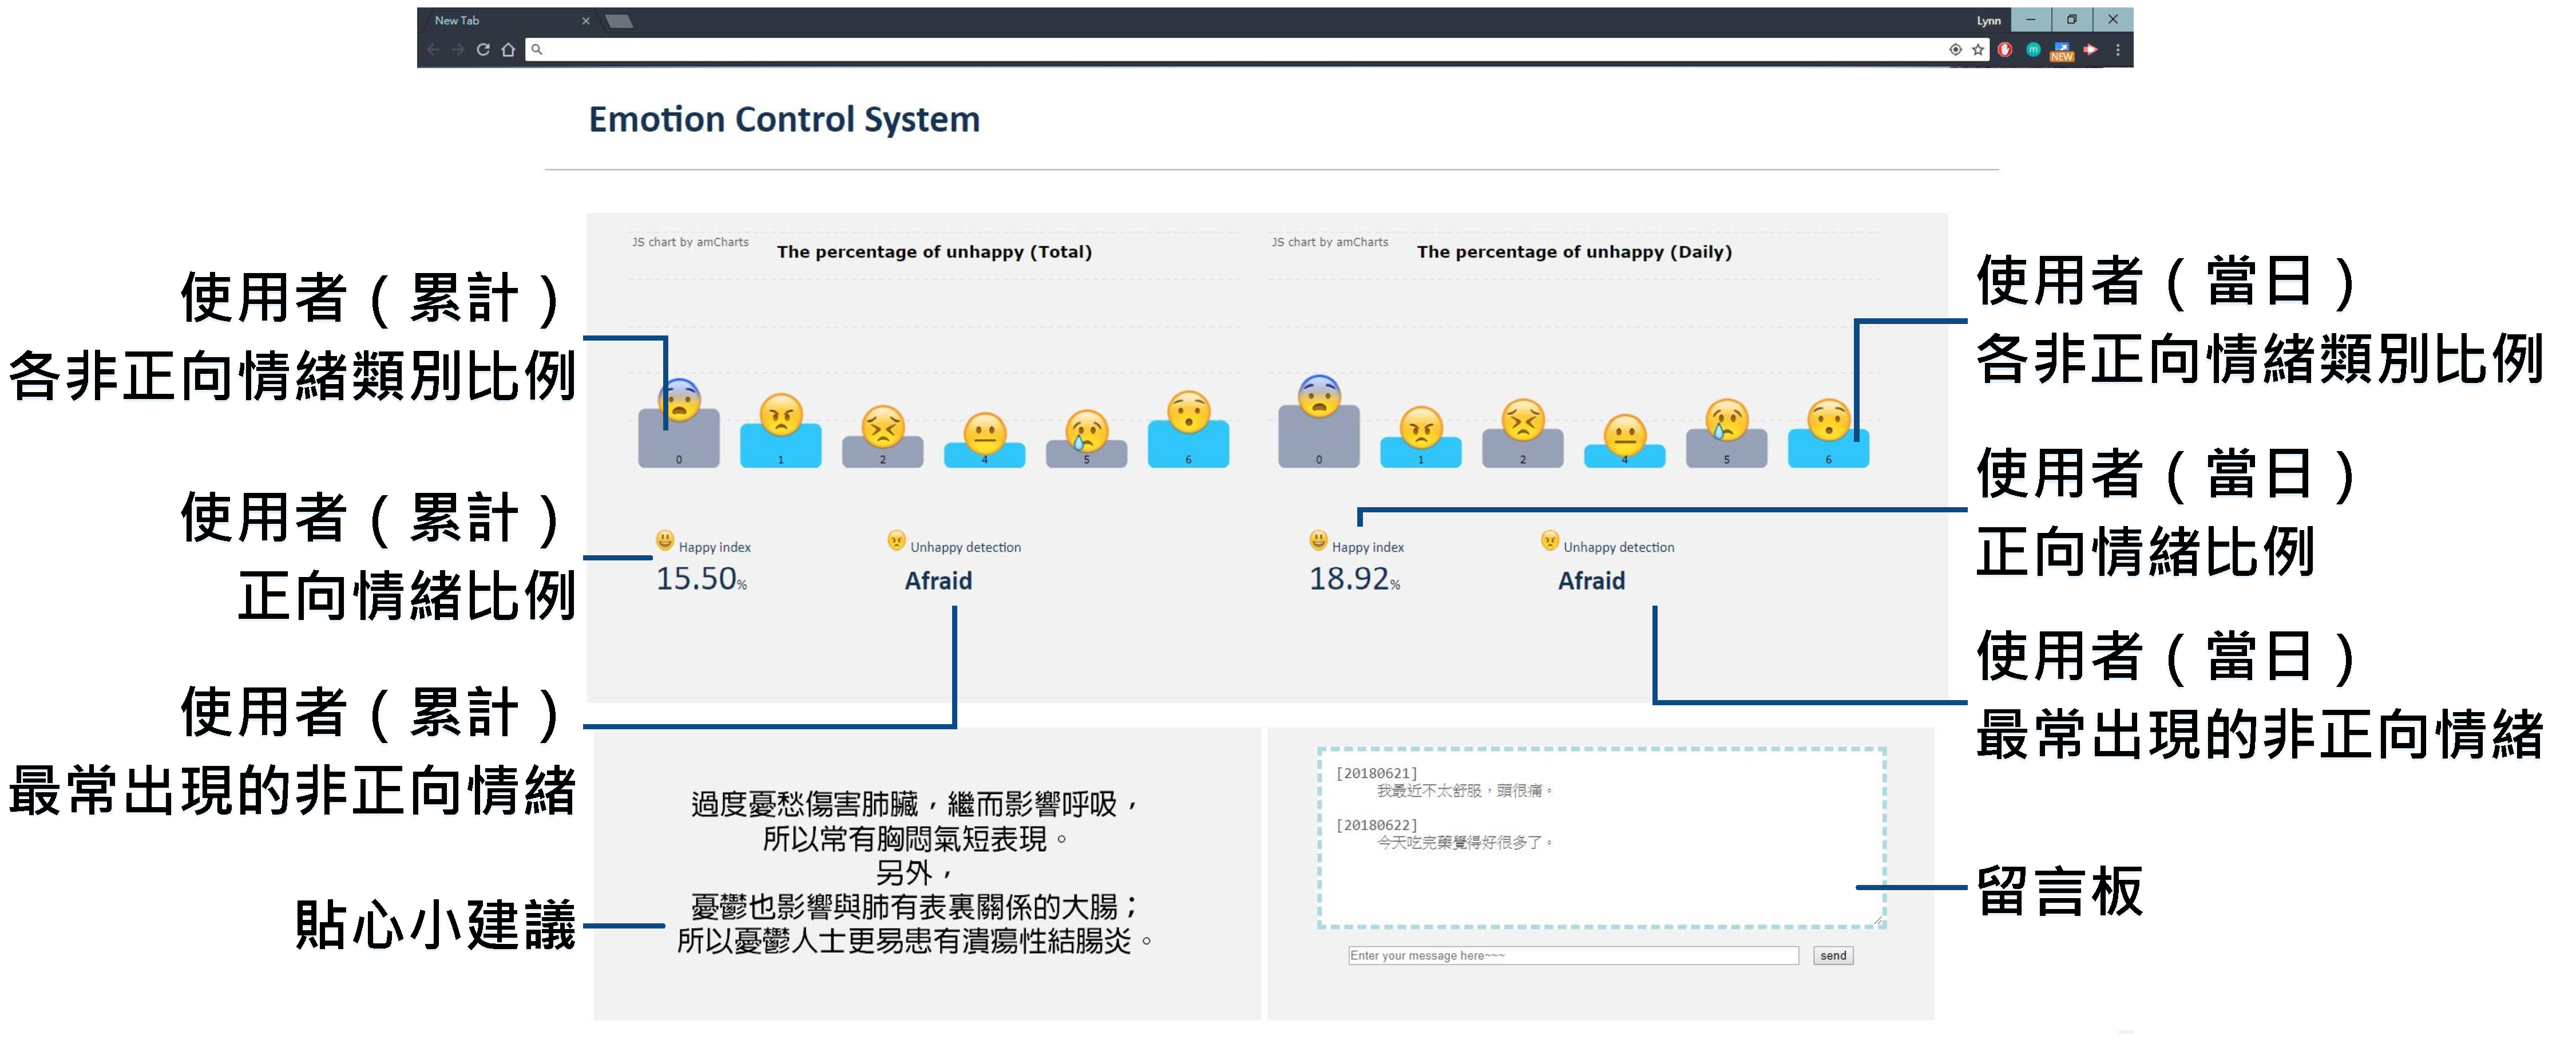
\includegraphics[width=1\textwidth]{./figs/Web.pdf}
\end{center}
\caption{伺服器端:雲端心靈陪伴分析整合平台示例圖。}
\label{fig:webframework}
\end{figure}
\end{itemize}

%$<$Provide a short description of the feature and indicate whether it is of 
%High, Medium, or Low priority. You could also include specific priority 
%component ratings, such as benefit, penalty, cost, and risk (each rated on a 
%relative scale from a low of 1 to a high of 9).$>$

\subsection{UML使用者案例圖表}
$<$List the sequences of user actions and system responses that stimulate the 
behavior defined for this feature. These will correspond to the dialog elements 
associated with use cases.$>$

\subsection{功能性需求}
$<$Itemize the detailed functional requirements associated with this feature.  
These are the software capabilities that must be present in order for the user 
to carry out the services provided by the feature, or to execute the use case.  
Include how the product should respond to anticipated error conditions or 
invalid inputs. Requirements should be concise, complete, unambiguous, 
verifiable, and necessary. Use “TBD” as a placeholder to indicate when necessary 
information is not yet available.$>$

$<$Each requirement should be uniquely identified with a sequence number or a 
meaningful tag of some kind.$>$


\chapter{其他非功能性需求}

\section{性能需求}

\begin{center}  
\begin{tabular}{|l| p{10cm}|}  
\hline  
非功能性需求 & 非功能性需求描述   \\ \hline  
偵測時間 & 情緒偵測應在0.3秒內即時完成    \\ \hline  
高準確率 & 情緒辨識系統準確率達95\%以上 \\ \hline
使用方便 &病人可與感測器設備保持30公分以上距離,不需配戴任何裝置,及繁瑣的操作步驟,便能直接蒐集病人的情緒變化,方便實際使用 \\ \hline
清楚呈現 & 本系統提供之分析整合平台,將雲端資料庫中的數據透過直方圖方式視覺化呈現於網頁上,得以清楚呈現病人非正向情緒之情形 \\ \hline
隨處皆可察看網頁平台 & 只要身邊有可瀏覽網頁之設備,便可以透過瀏覽器,使用本系統所提供之分析整合平台 \\ \hline

\end{tabular}  
\end{center}  

\section{safety需求}
$<$Specify those requirements that are concerned with possible loss, damage, or 
harm that could result from the use of the product. Define any safeguards or 
actions that must be taken, as well as actions that must be prevented. Refer to 
any external policies or regulations that state safety issues that affect the 
product’s design or use. Define any safety certifications that must be 
satisfied.$>$

\section{Security需求}
$<$Specify any requirements regarding security or privacy issues surrounding use 
of the product or protection of the data used or created by the product. Define 
any user identity authentication requirements. Refer to any external policies or 
regulations containing security issues that affect the product. Define any 
security or privacy certifications that must be satisfied.$>$

\section{軟體優良特質}
目前一般穩定情緒方法有兩種:

\begin{itemize}
\item[一、]{尋求心理諮詢師:}

諮詢師利用專業,在一對一的方式下,引導病人舒緩甚至是消除非正向情緒,並且給予適當的建議,所以價錢上相對來說是非常昂貴的。除此之外,尋求諮詢必須事先預約,導致當下的非正向情緒無法被立即的解決, 會有「非即時性」的問題。

\item[二、]{親朋好友:}

在心情不好的情況下,有時會不想和熟悉的人表達、抱怨,因為必須要顧及自己的面子,或者兩人之間朋友圈的重疊導致無法隨心所欲、暢所欲言,反而可能更壓抑自己,無法成功消除自己的非正向情緒;況且,非專業的人士提供的建議不一定是最適合的,甚至會導致非正向情緒更為惡劣。

\end{itemize}

基於上述兩種穩定情緒方法仍有不足之處,因此,我們提出本系統:基於即時情緒分析之心靈陪伴系統,使用深度學習產生訓練模型,將訓練資料進行情緒特徵抽取,再利用訓練完成的模型偵測病人情緒,獲得改善情緒之關鍵字,即時播放緩和情緒之音樂及心靈小語,舒緩病人非正向情緒。本系統具有以下三點特性:
\begin{itemize}
\item[1.]{專業性:}我們每個回饋、音樂,都是根據研究和專家證實過可以緩和情緒的回應,所以和親朋好友相比,此系統帶給病人情緒上的緩解是更立即且實用的。


\item[2.]{ 即時性:}在產生非正向情緒的當下立刻使用本系統,系統可以立即偵測病人的情緒,並且針對此情緒去做適當的回饋,而非像上述方法還需要事先預約,致使情緒不能立即紓解。


\item[3.] {後續追蹤:}上述提到,諮詢是尋求專業人士的協助,價格昂貴,導致可能久久才能諮詢一次。而使用此系統完全不會有這個問題,非正向情緒產生時,直接打開系統就可以使用,不會限制次數,也沒有價錢上的開銷。
\end{itemize}

搭配表\ref{lab:1},可以看出我們的系統同時擁有專業性、即時性和後續追蹤,相較其他兩個穩定情緒的方法我們系統不必花費高昂金額,尋求心理諮商師協助,也不會因顧及面子問題而無法暢所欲言,即可立即且有效緩和情緒。\\

\renewcommand{\arraystretch}{1.3} % 將表格行間距加大為原來的 1.2 倍
\begin{table}[!h]    
\centering
     \caption{各類穩定情緒方法之比較}
 \resizebox{0.48\textwidth}{!}{
 \begin{tabular}{|c|c|c|c|}\hline
 \diagbox[width=14em]{方法}{特性} & 專業性 & 即時性   &後續追蹤      \\\hline
    心理諮詢師   &○      & ×  & ×      \\\hline
    親朋好友      & ×    & ○  & Δ      \\\hline
    本系統                       & ○             & ○       & ○        \\\hline
    \end{tabular}}
\label{lab:1}
\end{table}

\section{商業規範}
$<$List any operating principles about the product, such as which individuals or 
roles can perform which functions under specific circumstances. These are not 
functional requirements in themselves, but they may imply certain functional 
requirements to enforce the rules.$>$


%\chapter{其他需求}
%$<$Define any other requirements not covered elsewhere in the SRS. This might 
%include database requirements, internationalization requirements, legal 
%requirements, reuse objectives for the project, and so on. Add any new sections 
%that are pertinent to the project.$>$
%
%\section{附錄A: 詞彙表}
%%see https://en.wikibooks.org/wiki/LaTeX/Glossary
%$<$Define all the terms necessary to properly interpret the SRS, including 
%acronyms and abbreviations. You may wish to build a separate glossary that spans 
%multiple projects or the entire organization, and just include terms specific to 
%a single project in each SRS.$>$
%
%\section{附錄B: 分析模組}
%$<$Optionally, include any pertinent analysis models, such as data flow 
%diagrams, class diagrams, state-transition diagrams, or entity-relationship 
%diagrams.$>$
%
%\section{附錄C: 待定列表}
%$<$Collect a numbered list of the TBD (to be determined) references that remain 
%in the SRS so they can be tracked to closure.$>$

%\section{Purpose}
%$<$Identify the product whose software requirements are specified in this 
%document, including the revision or release number. Describe the scope of the 
%product that is covered by this SRS, particularly if this SRS describes only 
%part of the system or a single subsystem.$>$
%
%\section{Document Conventions}
%$<$Describe any standards or typographical conventions that were followed when 
%writing this SRS, such as fonts or highlighting that have special significance.  
%For example, state whether priorities  for higher-level requirements are assumed 
%to be inherited by detailed requirements, or whether every requirement statement 
%is to have its own priority.$>$
%
%\section{Intended Audience and Reading Suggestions}
%$<$Describe the different types of reader that the document is intended for, 
%such as developers, project managers, marketing staff, users, testers, and 
%documentation writers. Describe what the rest of this SRS contains and how it is 
%organized. Suggest a sequence for reading the document, beginning with the 
%overview sections and proceeding through the sections that are most pertinent to 
%each reader type.$>$
%
%\section{Project Scope}
%$<$Provide a short description of the software being specified and its purpose, 
%including relevant benefits, objectives, and goals. Relate the software to 
%corporate goals or business strategies. If a separate vision and scope document 
%is available, refer to it rather than duplicating its contents here.$>$
%
%\section{References}
%$<$List any other documents or Web addresses to which this SRS refers. These may 
%include user interface style guides, contracts, standards, system requirements 
%specifications, use case documents, or a vision and scope document. Provide 
%enough information so that the reader could access a copy of each reference, 
%including title, author, version number, date, and source or location.$>$

%
%\chapter{創新及創意}
%\vspace{-1cm}
%目前一般穩定情緒方法有兩種:
%
%\begin{itemize}
%\item[一、]{尋求心理諮詢師:}
%
%諮詢師利用專業,在一對一的方式下,引導病人舒緩甚至是消除負面情緒,並且給予適當的建議,所以價錢上相對來說是非常昂貴的。除此之外,尋求諮詢必須事先預約,導致當下的負面情緒無法被立即的解決, 會有「非即時性」的問題。
%
%\item[二、]{親朋好友:}
%
%在心情不好的情況下,有時會不想和熟悉的人表達、抱怨,因為必須要顧及自己的面子,或者兩人之間朋友圈的重疊導致無法隨心所欲、暢所欲言,反而可能更壓抑自己,無法成功消除自己的負面情緒;況且,非專業的人士提供的建議不一定是最適合的,甚至會導致負面情緒更為惡劣。
%
%\end{itemize}
%
%基於上述兩種穩定情緒方法仍有不足之處,因此,我們提出本系統:基於即時情緒分析之心靈陪伴系統,使用深度學習產生訓練模型,將訓練資料進行情緒特徵抽取,再利用訓練完成的模型偵測病人情緒,獲得改善情緒之關鍵字,即時播放緩和情緒之音樂及心靈小語,舒緩病人負面情緒。本系統具有以下三點特性:
%\begin{itemize}
%\item[1.]{ 即時性:}在產生負面情緒的當下立刻使用本系統,系統可以立即偵測病人的情緒,並且針對此情緒去做適當的回饋,而非像上述方法還需要事先預約,致使情緒不能立即紓解。
%
%\item[2.]{重複使用性:}上述提到,諮詢是尋求專業人士的協助,價格昂貴,導致可能久久才能諮詢一次。而使用此系統完全不會有這個問題,負面情緒產生時,直接打開系統就可以使用,不會限制次數,也沒有價錢上的開銷。
%
%\item[3.] {專業性:}我們每個回饋、音樂,都是根據研究和專家證實過可以緩和情緒的回應,所以和親朋好友相比,此系統帶給病人情緒上的緩解是更立即且實用的。
%\end{itemize}
%
%搭配下表\ref{lab:1},可以看出我們的系統同時擁有即時性、重複使用性和專業性,相較其他兩個穩定情緒的方法我們系統不必花費高昂金額,尋求心理諮商師協助,也不會因顧及面子問題而無法暢所欲言,即可立即且有效緩和情緒。\\
%
%\renewcommand{\arraystretch}{1.3} % 將表格行間距加大為原來的 1.2 倍
%\begin{table}[!h]    
%\centering
%     \caption{各類穩定情緒方法之比較}
%	\resizebox{0.48\textwidth}{!}{
% \begin{tabular}{|c|c|c|c|}\hline
%	\diagbox[width=14em]{方法}{特性}	& 重複使用性	& 即時性	  & 專業性   	 \\\hline
%    心理諮詢師			& ×  		& × 	& ○	       \\\hline
%    親朋好友   			& ○  		& ○ 	& ×      \\\hline
%    本系統                       & ○             & ○       & ○        \\\hline
%    \end{tabular}}
%\label{lab:1}
%\end{table}

%\chapter{作品介紹}
%\vspace{-1cm}
%$~~~$根據國內〈科學發展〉期刊的相關研究發現,音樂可以產生催產素,以減低焦慮與恐懼,有效改善情緒,因此,本系統:基於即時情緒分析之心靈陪伴系統,應用於醫療系統的照護病患機制,本專案系統主要分為兩部份,分別為使用者端和伺服器端,使用者端為情緒偵測演算法及情緒緩和機制,伺服器端則為雲端心靈陪伴分析整合平台,如圖\ref{fig:framework},概略說明如下:
%
%%%%%圖要改
%\begin{figure}[!h]
%\begin{center}
%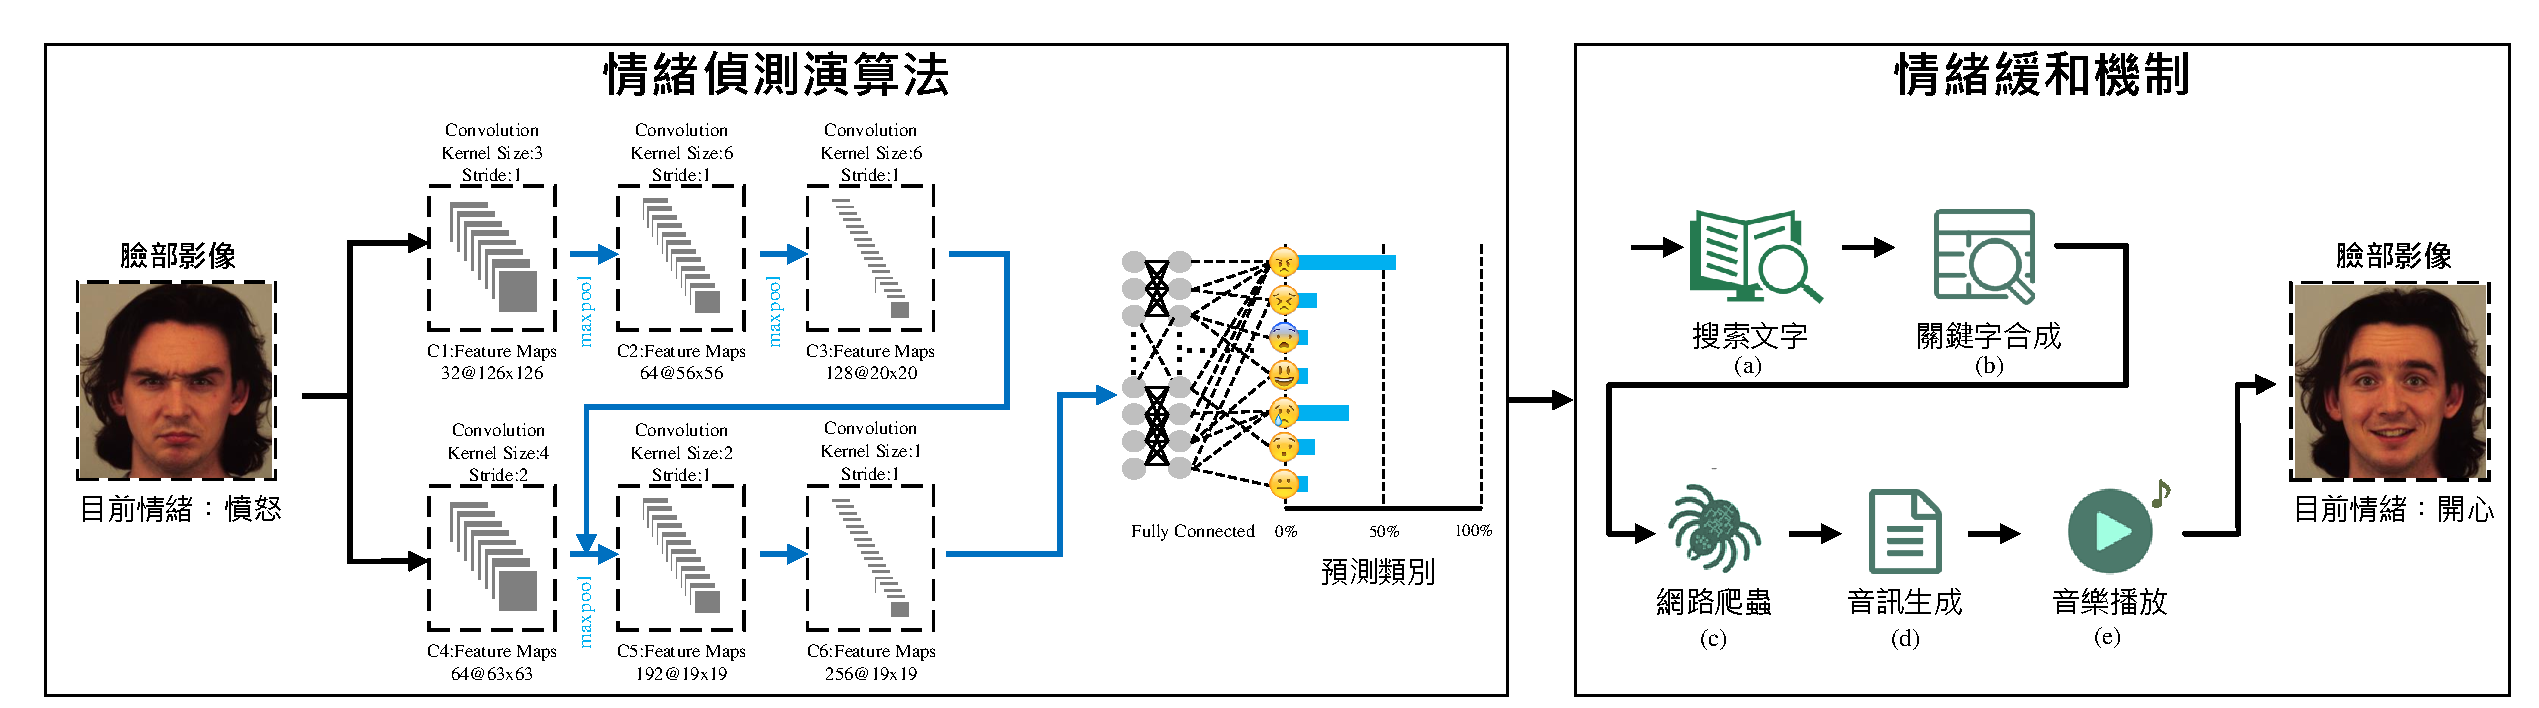
\includegraphics[width=1\textwidth]{./figs/framework.pdf}
%\end{center}
%\caption{非接觸式準確且即時駕駛情緒偵測演算法架構圖。}
%\label{fig:framework}
%\end{figure}
%%%%%%%%%%%%%%%%%%%%%%%%%%%%%%%
%\begin{itemize}
%\item[1.]{\begin{bfseries}{使用者端:}\end{bfseries}}
%
%\begin{itemize}
%\item[a.]{\begin{bfseries}{情緒偵測演算法:}\end{bfseries}}
%
%我們為避免病人因極端負面情緒,持續影響心理、生理,進而導致不可預期的危害,我們利用深度學習的卷積神經網路CNN,由1個輸入層、6個卷積層(Convolution layer)、3個池化層(Pooling layer)、1個全連接層(Fully Connected)和1個輸出層所構成,來訓練情緒辨識模型,偵測病人情緒。由於情緒的時間性變化,我們亦進行兩階段的Voting機制,第一階段為篩選出病人可能的情緒,第二階段為避免病人因為短時間臉部抽動(如:打哈欠),導致誤判情緒,透過上述兩階段的Voting後,得出最準確的病人情緒判斷。\\
%
%\item[b.]{\begin{bfseries}{情緒緩和機制:}\end{bfseries}}
%
%透過情緒偵測演算法,得出的病人情緒後,即時抓取能有效改善病人當下情緒的音樂並播放,使病人情緒緩和,避免病人因極端負面情緒,導致影響心理,使病情不易痊癒、影響治療過程。因此,我們分為五個步驟達成,包括:搜索文字、關鍵字合成、網路爬蟲、音訊生成、以及音樂播放等五個步驟。\\
%
%\begin{itemize}
%\item[(Ⅰ)]{\begin{bfseries}{搜索文字:}\end{bfseries}}
%
%當抓取到病人情緒後,我們隨機搜索一組預先設定的回應文字,如表\ref{lab:searchtext}所示,利用語音播放,回應正向語句,鼓勵病人。\\
%
%\renewcommand{\arraystretch}{1.2} 
%\renewcommand{\multirowsetup}{\centering}
%
%\begin{table}[h]
%\caption{搜索文字表}
%    \centering
%\begin{tabular}{|*{4}{r|}}
%\hline
%\multicolumn{1}{|c|}{情緒}
%& \multicolumn{3}{c|}{回應字} \\\hline
%\multicolumn{1}{|c}{憤怒}&\multicolumn{1}{|c}{奧特曼,你別氣了,…}&\multicolumn{1}{|c}{……}&\multicolumn{1}{|c|}{沒有什麼事情是十全…} \\\hline
%\multicolumn{1}{|c}{悲傷}&\multicolumn{1}{|c}{讓我陪你一起面對,…}&\multicolumn{1}{|c}{……}&\multicolumn{1}{|c|}{我知道現在的你情緒…} \\\hline
%\multicolumn{1}{|c}{驚嚇}&\multicolumn{1}{|c}{偉大的哈利來幫你了…}&\multicolumn{1}{|c}{……}&\multicolumn{1}{|c|}{你心裡一定很不好受…}\\\hline
%\multicolumn{1}{|c}{憂慮}&\multicolumn{1}{|c}{如果你願意說,我隨…}&\multicolumn{1}{|c}{……}&\multicolumn{1}{|c|}{遇到什麼是很心煩嗎…}\\\hline
%\multicolumn{1}{|c}{厭惡}&\multicolumn{1}{|c}{燒毀,燒毀,斷開魂…}   &\multicolumn{1}{|c}{……}   &\multicolumn{1}{|c|}{偶爾深呼吸,心情更… }\\\hline
%\multicolumn{1}{|c}{無表情}&\multicolumn{1}{|c}{有一個爸爸帶四歲的…}   &\multicolumn{1}{|c}{……}   &\multicolumn{1}{|c|}{我來講個笑話給你聽…}\\\hline
%\multicolumn{1}{|c}{開心}&\multicolumn{1}{|c}{你開心ya,我開心ya…}   &\multicolumn{1}{|c}{……}   &\multicolumn{1}{|c|}{今天心情不錯!繼續保…}\\\hline
%\end{tabular}
%\label{lab:searchtext}
%\end{table}
%
%\item[(Ⅱ)]{\begin{bfseries}{關鍵字合成:}\end{bfseries}}
%
%我們根據設定的查找表(Lookup Table)來合成網路爬蟲關鍵字,如表\ref{lab:2}所示(放關鍵字合成的表)。其中,如果是偵測到病人的情緒為「憤怒」,會查找到可能的關鍵字有「古典樂放鬆」、「古典樂輕快」、「流行歌輕快」等,以找尋放鬆、輕快的音訊資料,如圖\ref{fig:framework}右半部(b)所示。\\
%
%\renewcommand{\arraystretch}{1.2} 
%\renewcommand{\multirowsetup}{\centering}
%\begin{table}[h]
%\caption{關鍵字合成表}
%    \centering
%\begin{tabular}{|*{4}{r|}}
%\hline
%\multicolumn{1}{|c|}{情緒}
%& \multicolumn{3}{c|}{關鍵字} \\\hline
%\multicolumn{1}{|c}{憤怒}&\multicolumn{1}{|c}{古典樂放鬆}&\multicolumn{1}{|c}{古典樂輕快}&\multicolumn{1}{|c|}{流行歌輕快} \\\hline
%\multicolumn{1}{|c}{悲傷}&\multicolumn{1}{|c}{療癒音樂}&\multicolumn{1}{|c}{交響樂輕快}&\multicolumn{1}{|c|}{交響曲振奮} \\\hline
%\multicolumn{1}{|c}{驚嚇}&\multicolumn{1}{|c}{鋼琴輕音樂}&\multicolumn{1}{|c}{背景音樂輕鬆}&\multicolumn{1}{|c|}{背景音樂抒情}\\\hline
%\multicolumn{1}{|c}{厭惡}&\multicolumn{1}{|c}{純音樂提神}&\multicolumn{1}{|c}{交響樂震撼}&\multicolumn{1}{|c|}{背景音樂震撼}\\\hline
%\multicolumn{1}{|c}{焦慮}&\multicolumn{1}{|c}{古典樂振奮}   &\multicolumn{1}{|c}{舒緩音樂}   &\multicolumn{1}{|c|}{振奮人心音樂}\\\hline
%\multicolumn{1}{|c}{無表情}&\multicolumn{1}{|c}{背景音樂輕鬆}   &\multicolumn{1}{|c}{背景音樂抒情}   &\multicolumn{1}{|c|}{流行歌輕快}\\\hline
%\multicolumn{1}{|c}{開心}&\multicolumn{1}{|c}{清音樂自然}   &\multicolumn{1}{|c}{鋼琴輕音樂}   &\multicolumn{1}{|c|}{背景音樂自然}\\\hline
%\end{tabular}
%\label{lab:2}
%\end{table}
%
%\item[(Ⅲ)]{\begin{bfseries}{網路爬蟲:}\end{bfseries}}
%
%利用關鍵字合成,使用網路爬蟲,抓取有效改善病人當下情緒的音樂,我們採用HTTP Request技術,以及requests、urllib2、 BeautifulSoup 、lxml、 youtube-dl等軟體開發套件,根據上述的關鍵字檢索結果,從網絡上抓取最新最即時的音訊資料,如圖\ref{fig:framework}右半部(c)所示。\\
%
%\item[(Ⅳ)]{\begin{bfseries}{音訊生成:}\end{bfseries}}
%
%當我們抓取到音訊資料後,通過Python的Requests及 BeautifulSoup技術,來下載檔案,使音訊生成,如圖\ref{fig:framework}右半部(d)所示。\\
%
%\item[(Ⅴ)]{\begin{bfseries}{音樂播放:}\end{bfseries}}
%
%當我們生成音訊資料後,使用omxplayer套件,將音訊播放給病人收聽,改善病人當下的情緒,如圖\ref{fig:framework}右半部(e)所示。\\
%
%\end{itemize}
%
%根據以上五個步驟,即可完成情緒緩和機制,藉此避免病人因極端負面情緒,導致影響病情,賦予病人積極、正面的動力。\\
%
%
%\end{itemize}
%\item[2.]{\begin{bfseries}{伺服器端:}\end{bfseries}}\\
%\begin{bfseries}雲端心靈陪伴分析整合平台:\end{bfseries}
%
%透過情緒緩和機制分析過後,我們導入分析後的負面情緒類別,設計一雲端心靈陪伴分析整合平台,如圖攵所示,以提供視覺化情緒統計的服務。如此一來,一般民眾能透過網頁,查詢自己的歷史狀況,以及分析統計結果;車隊管理人能透過該車隊的統計結果,知道哪些路段及哪些成員最容易分心駕駛,進行駕駛行為矯正。
%\end{itemize}


%\section{User Interfaces}
%$<$Describe the logical characteristics of each interface between the software 
%product and the users. This may include sample screen images, any GUI standards 
%or product family style guides that are to be followed, screen layout 
%constraints, standard buttons and functions (e.g., help) that will appear on 
%every screen, keyboard shortcuts, error message display standards, and so on.  
%Define the software components for which a user interface is needed. Details of 
%the user interface design should be documented in a separate user interface 
%specification.$>$
%
%\section{Hardware Interfaces}
%$<$Describe the logical and physical characteristics of each interface between 
%the software product and the hardware components of the system. This may include 
%the supported device types, the nature of the data and control interactions 
%between the software and the hardware, and communication protocols to be 
%used.$>$
%
%\section{Software Interfaces}
%$<$Describe the connections between this product and other specific software 
%components (name and version), including databases, operating systems, tools, 
%libraries, and integrated commercial components. Identify the data items or 
%messages coming into the system and going out and describe the purpose of each.  
%Describe the services needed and the nature of communications. Refer to 
%documents that describe detailed application programming interface protocols.  
%Identify data that will be shared across software components. If the data 
%sharing mechanism must be implemented in a specific way (for example, use of a 
%global data area in a multitasking operating system), specify this as an 
%implementation constraint.$>$
%
%\section{Communications Interfaces}
%$<$Describe the requirements associated with any communications functions 
%required by this product, including e-mail, web browser, network server 
%communications protocols, electronic forms, and so on. Define any pertinent 
%message formatting. Identify any communication standards that will be used, such 
%as FTP or HTTP. Specify any communication security or encryption issues, data 
%transfer rates, and synchronization mechanisms.$>$

%
%\chapter{操作環境說明}
%\begin{itemize}
%\item[(1)]{\begin{bfseries}{操作系統:}Windows 10\end{bfseries}}
%\item[(2)]{\begin{bfseries}{程式撰寫平台:}Pycharm 2016.3.2\end{bfseries}}
%\item[(3)]{\begin{bfseries}{操作環境:}Python3.5.0 以上\end{bfseries}}
%\item[(4)]{\begin{bfseries}{使用套件:}NumPy、OpenCV、Tensorflow、Keras、BeautifulSoup、
% youtube_dl、lxml、ffmpeg\end{bfseries}}
%\item[(5)]{\begin{bfseries}{相關配件:}具備藍芽功能之音響及攝影機\end{bfseries}}
%\item[(6)]{\begin{bfseries}{網路:}無線網路卡或手機 wifi\end{bfseries}}
%
%\end{itemize}
%\chapter{Other Nonfunctional Requirements}
%
%\section{Performance Requirements}
%$<$If there are performance requirements for the product under various 
%circumstances, state them here and explain their rationale, to help the 
%developers understand the intent and make suitable design choices. Specify the 
%timing relationships for real time systems. Make such requirements as specific 
%as possible. You may need to state performance requirements for individual 
%functional requirements or features.$>$
%
%\section{Safety Requirements}
%$<$Specify those requirements that are concerned with possible loss, damage, or 
%harm that could result from the use of the product. Define any safeguards or 
%actions that must be taken, as well as actions that must be prevented. Refer to 
%any external policies or regulations that state safety issues that affect the 
%product’s design or use. Define any safety certifications that must be 
%satisfied.$>$
%
%\section{Security Requirements}
%$<$Specify any requirements regarding security or privacy issues surrounding use 
%of the product or protection of the data used or created by the product. Define 
%any user identity authentication requirements. Refer to any external policies or 
%regulations containing security issues that affect the product. Define any 
%security or privacy certifications that must be satisfied.$>$
%
%\section{Software Quality Attributes}
%$<$Specify any additional quality characteristics for the product that will be 
%important to either the customers or the developers. Some to consider are: 
%adaptability, availability, correctness, flexibility, interoperability, 
%maintainability, portability, reliability, reusability, robustness, testability, 
%and usability. Write these to be specific, quantitative, and verifiable when 
%possible. At the least, clarify the relative preferences for various attributes, 
%such as ease of use over ease of learning.$>$
%
%\section{Business Rules}
%$<$List any operating principles about the product, such as which individuals or 
%roles can perform which functions under specific circumstances. These are not 
%functional requirements in themselves, but they may imply certain functional 
%requirements to enforce the rules.$>$
%
%
%\chapter{Other Requirements}
%$<$Define any other requirements not covered elsewhere in the SRS. This might 
%include database requirements, internationalization requirements, legal 
%requirements, reuse objectives for the project, and so on. Add any new sections 
%that are pertinent to the project.$>$
%
%\section{Appendix A: Glossary}
%%see https://en.wikibooks.org/wiki/LaTeX/Glossary
%$<$Define all the terms necessary to properly interpret the SRS, including 
%acronyms and abbreviations. You may wish to build a separate glossary that spans 
%multiple projects or the entire organization, and just include terms specific to 
%a single project in each SRS.$>$
%
%\section{Appendix B: Analysis Models}
%$<$Optionally, include any pertinent analysis models, such as data flow 
%diagrams, class diagrams, state-transition diagrams, or entity-relationship 
%diagrams.$>$
%
%\section{Appendix C: To Be Determined List}
%$<$Collect a numbered list of the TBD (to be determined) references that remain 
%in the SRS so they can be tracked to closure.$>$

\end{document}
